% Author: Nils Pukropp
% E-Mail: nils.pukropp@student.kit.edu
% License: MIT
\documentclass[aspectratio=169]{beamer}

\usepackage{fontspec}

\usetheme{metropolis}

\setmonofont[
  Contextuals={Alternate},
  Ligatures = TeX,
]{FiraCode Nerd Font}

\newcommand{\HUMONGOUS}{\Huge}

\usepackage{booktabs}
\usepackage[scale=2]{ccicons}

\usepackage{color}

\definecolor{linkcolor}{HTML}{EE0E61}

\hypersetup{
  colorlinks=true,
  linkcolor= {linkcolor},
  urlcolor= {linkcolor},
  bookmarks={true}
}

\definecolor{stringcolor}{RGB}{139,233,253}
\definecolor{commentcolor}{RGB}{189,147,249}
\definecolor{alertcolor}{RGB}{255,85,85}
\definecolor{keywordcolor}{RGB}{255 184 108}
\definecolor{FGround}{RGB}{248,248,242}
\definecolor{BGround}{RGB}{40,42,54}
\definecolor{classcolor}{HTML}{EE0E61}
\definecolor{numbercolor}{HTML}{6897bb}
\definecolor{darkgray}{HTML}{2b2b2b}
\definecolor{nicegreen}{HTML}{50fa7b}

\usepackage{listings}
\lstset{
  backgroundcolor=\color{BGround},
  language=Java,
  showspaces=false,
  showtabs=false,
  breaklines=true,
  columns = flexible,
  showstringspaces=true,
  breakatwhitespace=true,
  keywordstyle=\color{keywordcolor},
  morekeywords={enum},
  commentstyle=\color{commentcolor},
  stringstyle=\color{stringcolor},
  basicstyle=\footnotesize\ttfamily\color{FGround},
  numbers=left,
  numbersep=5pt,
  numberstyle=\color{numbercolor},
  captionpos=b,
  extendedchars=true,
  tabsize=2,
  escapeinside={\%*}{*)},
  moredelim=[is][\color{classcolor}]{@@c}{@@}
}

\usepackage{pgfplots}
\usepgfplotslibrary{dateplot}
\pgfplotsset{compat=1.16}

\usepackage{xspace}
\usepackage{multicol}

\title{\color{classcolor}Tutorium Woche 7 - Termin 1}
\subtitle{Tipps Abschlussaufgaben}
\date{\today}
\author{Nils Pukropp}
\institute{INSTITUT FÜR PROGRAMMSTRUKTUREN UND DATENORGANISATION}
\titlegraphic{\hfill
\includegraphics[height=1.5cm]{../logos/KIT-Logo.png}}
\metroset{block=fill}
\setbeamercolor{background canvas}{bg=darkgray}
\setbeamercolor{normal text}{fg=FGround, bg=darkgray}
\setbeamercolor{alerted text}{fg=alertcolor, bg=darkgray}
\setbeamercolor{example text}{fg=commentcolor, bg=darkgray}
\setbeamercolor{progressbar in foot}{fg=classcolor}
\setbeamercolor{frametitle}{bg=BGround, fg=FGround}


\begin{document}
\maketitle

\begin{frame}{Übersicht}
  \setbeamertemplate{section in toc}[sections numbered]
  \tableofcontents[hideallsubsections]
\end{frame}

\section{Vorstellung}
\begin{frame}[fragile]{Vorstellung}
  \begin{block}{Über mich}
  \begin{itemize}
    \item Nils Pukropp, 21 Jahre
    \begin{itemize}
      \item Informatik Bachelor im 4. Semester
    \end{itemize}
    \item E-Mail: \href{mailto:nils.pukropp@student.kit.edu}{nils.pukropp@student.kit.edu}
    \item Discord: \href{https://discord.gg/6GpaFE8w4y}{KIT Mathe Info}
  \end{itemize}
\end{block}
\end{frame}

\begin{frame}[fragile]{Vorstellung}
 \begin{columns}[T,onlytextwidth]
    \column{0.5\textwidth}
      \begin{block}{Regeln/Empfehlungen für MS Teams}
        \begin{itemize}
          \item Ton aus/Webcam an (falls, vorhanden, Alternative: droidcam)
          \item De-Anonymisierung aktiviert
          \item Fragen stellen \begin{itemize}
            \item einfach los fragen (einfach zwischen rein)
            \item oder Hand heben
            \item Duzen ist erwünscht
          \end{itemize}
        \end{itemize}
      \end{block}
    \column{0.05\textwidth}
    \column{0.5\textwidth}
      
\includegraphics[scale=0.4]{../images/questions-meme.jpg}
  \end{columns}

\end{frame}

\section{Organisatorisches}
\begin{frame}[fragile]{Organisatorisches}
  \begin{alertblock}{Organisatorisches}
    \begin{itemize}
      \item Schauen ob man den Übungsschein hat
      \item Abschlussaufgabe 1 \begin{itemize}
        \item \color{nicegreen}Ausgabe: \color{FGround} 12. Juli, 13 Uhr
        \item \color{numbercolor} Artemis: \color{FGround} 26. Juli, 13 Uhr
        \item \color{alertcolor}Deadline: \color{FGround} 08. August, 06 Uhr
      \end{itemize}
      \item Abschlussaufgabe 2 \begin{itemize}
        \item \color{nicegreen}Ausgabe: \color{FGround} 26. Juli, 13 Uhr
        \item \color{numbercolor} Artemis: \color{FGround} 09. August, 13 Uhr
        \item \color{alertcolor}Deadline: \color{FGround} 24. August, 06 Uhr
      \end{itemize}
    \end{itemize}
  \end{alertblock}
  \begin{block}{Abschlussaufgaben}
    Nehmt euch genügend Zeit für die Abschlussaufgaben, also fangt nicht erst ein paar Tage vor Abgabe an.
  \end{block}
\end{frame}

\section{Interaktive Benutzerschnittstellen}
\subsection{Enum als Benutzerschnittstelle}
\begin{frame}{Enum als Benutzerschnittstelle}
  \begin{block}{Vorprogrammieren in VSCode}
    Lösung wird im Ilias hochgeladen! Ihr könnt einfach zuschauen und Fragen stellen
  \end{block}
\end{frame}

\subsection{Beispiel Musterlösung Blatt 5.}
\begin{frame}{Beispiel Musterlösung Blatt 5.}
  Siehe Musterlösung
\end{frame}

\subsection{Alternative: Command-Pattern}
\begin{frame}{Alternative: Command-Pattern}
  \begin{block}{Vorprogrammieren in VSCode}
    Lösung wird im Ilias hochgeladen! Ihr könnt einfach zuschauen und Fragen stellen
  \end{block}
\end{frame}

\section{Tipps für die Abschlussaufgaben}

\subsection{Namenskonventionen}
\begin{frame}[fragile]{Namenskonventionen}
  \begin{block}{Attribut- und Methodennamen}
    lowerCamelCase \linebreak
    \pause
    \color{nicegreen}Do.\color{FGround}
    \begin{lstlisting}[numbers=none]
private int turnCount;
public void addToken(@@cToken@@ newToken) {...
    \end{lstlisting}
    \pause
    \color{alertcolor}Don't.\color{FGround}
    \begin{lstlisting}[numbers=none]
private int n;
public void add(@@cToken@@ t) {...
    \end{lstlisting}
  \end{block}
\end{frame}


\begin{frame}[fragile]
  \begin{block}{Klassen und Interfaces}
    UpperCamelCase \linebreak
    \pause
    \color{nicegreen}Do.\color{FGround}
    \begin{lstlisting}[numbers=none]
public class @@cMain@@ {...
    \end{lstlisting}
    \pause
    \color{alertcolor}Don't.\color{FGround}
    \begin{lstlisting}[numbers=none]
public class @@cmain@@ {...
    \end{lstlisting}
  \end{block}

  \begin{block}{Konstanten}
    UPPER\_CASE\_WITH\_UNDERSCORE \linebreak
    \pause
    \color{nicegreen}Do.\color{FGround}
    \begin{lstlisting}[numbers=none]
public static final int BOARD_WIDTH = 16;
    \end{lstlisting}
    \pause
    \color{alertcolor}Don't.\color{FGround}
    \begin{lstlisting}[numbers=none]
public static final int Width = 16;
    \end{lstlisting}
  \end{block}
\end{frame}

\subsection{JavaDocs}
\begin{frame}[fragile]{JavaDocs}
  \begin{block}{JavaDocs}
    Alle nicht-privaten Methoden, Konstanten (Auch Enums) und Klassenköpfe ausführlich dokumentieren! \\
    Besonders auf "Seiteneffekte" hinweisen. \linebreak
    \pause
    \color{nicegreen}Do.\color{FGround}
    \begin{lstlisting}[numbers=none]
/** 
 * Method to add a new data point. Updates 
 * the count and tells connected  
 * representation objects to update. 
 *
 * @param data  the data point to be added 
 */ 
void addDataPoint(@@cDataPoint@@ data) 
    \end{lstlisting}
  \end{block}
\end{frame}

\begin{frame}[fragile]
  \begin{block}{JavaDocs}
    \color{alertcolor}Don't.\color{FGround}
    \begin{lstlisting}[numbers=none]
/** 
 * add-Method.  
 */ 
void addDataPoint(@@cDataPoint@@ data)

/** 
 * @param data data
 * add-Method.  
 */ 
void addDataPoint(@@cDataPoint@@ data)
    \end{lstlisting}
  \end{block}
\end{frame}

\subsection{Magic Numbers}
\begin{frame}[fragile]{Magic Numbers}
  \begin{block}{Magic Numbers}
    Zahlen-Literale außer -1, 0, 1, 2 sollten in Variabeln oder Konstanten verpackt sein, damit man deren Bedeutung gleich erkennt.
    Das bietet sich auch für Ein-/Ausgabe Strings an. \linebreak
    \pause
    \color{nicegreen}Do.\color{FGround}
    \begin{lstlisting}[numbers=none]
public static final int DECK_SIZE = 52; 
for (int i = 0; i < DECK_SIZE; i++) { 
 ...
}
    \end{lstlisting}
    \pause
    \color{alertcolor}Don't.\color{FGround}
    \begin{lstlisting}[numbers=none]
for (int i = 0; i < 52; i++) { 
 ...
} 
    \end{lstlisting}
  \end{block}
\end{frame}

\subsection{Datenkapselung}
\begin{frame}[fragile]{Datenkapselung}
  \begin{block}{Datenkapselung}
    Attribute \textbf{private}, getter \& setter. Das gilt auch für Listen und Arrays! 
    Keine Implementierungsdetails verraten durch das herausgeben von ganzen Listen/Arrays. \linebreak
    \pause
    \color{nicegreen}Do.\color{FGround}
    \begin{lstlisting}[numbers=none]
private int speed; // km/h

public int getSpeedKmh() { return this.speed; }
public int getSpeedMph() { ... }
    \end{lstlisting}
    \pause
    \color{alertcolor}Don't.\color{FGround}
    \begin{lstlisting}[numbers=none]
public int speed; // km/h
    \end{lstlisting}
  \end{block}
\end{frame}

\subsection{Objektorientierung}
\begin{frame}[fragile]{Objektorientierung}
  \begin{block}{Objektorientierung}
    Gegen Interfaces statt konkreter Implementierung programmieren. \linebreak
    \pause
    \color{nicegreen}Do.\color{FGround}
    \begin{lstlisting}[numbers=none]
@@cList@@<@@cString@@> list = new @@cArrayList@@<>();
    \end{lstlisting}
    \pause
    \color{alertcolor}Don't.\color{FGround}
    \begin{lstlisting}[numbers=none]
@@cArrayList@@<@@cString@@> list = new @@cArrayList@@<>();
    \end{lstlisting}
  \end{block}
\end{frame}

\subsection{Seperation of Concerns, Static/Konstanten und Schachtelung}
\begin{frame}
  \begin{block}{Separation Of Concerns}
    \begin{itemize}
      \pause
      \item Pro Klasse nur passende Verantwortlichkeit / stark zusammenhängende Aktionen
      \pause
      \item z.B. ein Spielfeld kennt nur die eigene String-Rpräsentation (toString() !), hat aber keine Methoden zur Ausgabe.
    \end{itemize}
  \end{block}
  \pause
  \begin{block}{Static/Konstanten}
    \begin{itemize}
      \pause
      \item Konstanten sollten 
      \color{keywordcolor}public\color{FGround}, \color{keywordcolor}static \color{FGround} und \color{keywordcolor}final \color{FGround} sein.
      \pause
      \item Statische Methoden sind meistens allgemein brauchbare Methoden wie Math.random(), Stichwort Utility-Klasse
    \end{itemize}
  \end{block}
  \pause
  \begin{block}{Schachtelung}
    Methoden nicht zu tief schachteln! Schauen was man in Hilfsmethoden schreiben kann.
  \end{block}
\end{frame}

\begin{frame}[fragile]
  \begin{block}{If-Abfragen}
    \color{keywordcolor}if\color{FGround}-Abfragen lassen sich manchmal reduzieren, indem man sie "invertiert" \linebreak
    \pause
    \color{nicegreen}Do.\color{FGround}
    \begin{lstlisting}[numbers=none]
if (!outerCheck) { 
    return; 
} 
if (!innerCheck) { 
    return; 
} 
...
    \end{lstlisting}
    \pause
    \color{alertcolor}Don't.\color{FGround}
    \begin{lstlisting}[numbers=none]
if (outerCheck) { 
    if (innerCheck) { 
        ... 
    } 
}
    \end{lstlisting}
  \end{block}
\end{frame}

\subsection{Exceptions}
\begin{frame}{Exceptions}
  \begin{block}{Exceptions}
    \begin{itemize}
      \pause
      \item Sollten nicht den Kontrollfluss steuern (Ausnahme: z.B. \color{classcolor}NumberFormatException\color{FGround})
      \pause
      \item Generell: Keine \color{classcolor}RuntimeException\color{FGround}-Untertypen behandeln, sondern Fehler finden.
      \pause
      \item Exceptions bitte nach ihrem JavaDoc verwenden. Wenn keine passt eigene Exception schreiben und sinnvoll erben lassen. \linebreak
      Beliebte Kanidaten:
      \begin{itemize}
        \pause
        \item \href{https://docs.oracle.com/en/java/javase/16/docs/api/java.base/java/lang/IllegalArgumentException.html}{IllegalArgumentException}
        \pause
        \item \href{https://docs.oracle.com/en/java/javase/16/docs/api/java.base/java/lang/IllegalStateException.html}{IllegalStateException}
        \pause
        \item \href{https://docs.oracle.com/en/java/javase/16/docs/api/java.base/java/lang/ArithmeticException.html}{ArithmeticException}
      \end{itemize}
    \end{itemize}
  \end{block}
\end{frame}

\begin{frame}{Wann Fangen, wann nicht?}
  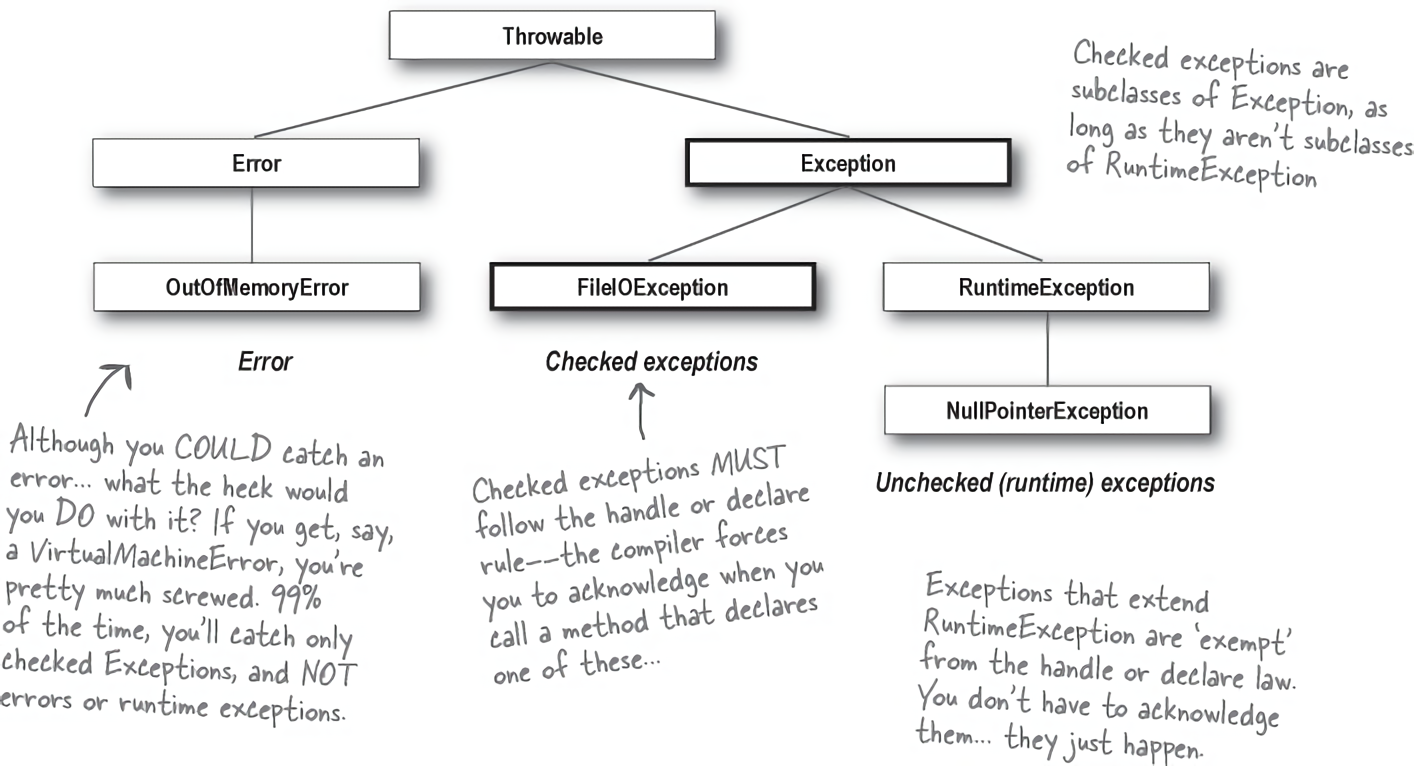
\includegraphics[scale=0.28]{../images/when_which_exception.png}
\end{frame}

\subsection{Erweiterbarkeit, Generics und Programmierstil}
\begin{frame}{Erweiterbarkeit/Generics und Stil}
  \begin{block}{Erweiterbarkeit \& Generics}
    \begin{itemize}
      \pause
      \item Bitte es nicht mit Erweiterbarkeit und Generics übertreiben!
      \pause
      \item Wenn ihr eine nicht-generische Lösung habt die aber sinnvoll objektorientiert ist, sollte das vollkommend in Ordnung sein.
    \end{itemize}
  \end{block}
  \pause
  \begin{block}{Programmierstil}
    \begin{itemize}
      \pause
      \item Lange \color{keywordcolor}if\color{FGround}-\color{keywordcolor}else\color{FGround}- oder \color{keywordcolor}switch\color{FGround}-statements
      sind tendenziell ein schlechtes Zeichen.
      \pause
      \item \color{keywordcolor}instanceOf \color{FGround} oder getClass() werden in Programmieren eigentlich nur in \textbf{equals(Object o)}, ... verwendet.
      Stichwort \textbf{Polymorphismus}
      \pause
      \item Nicht zu viele \color{keywordcolor}return\color{FGround}-statements. Stichwort Komplexität
    \end{itemize}
  \end{block}
\end{frame}

\subsection{Testen!}
\begin{frame}{\textbf{Und nicht vergessen!}}
  \pause
  \begin{center}\HUMONGOUS TESTEN!!! \end{center}
\end{frame}


\begin{frame}
  \begin{center}\HUMONGOUS Fragen?
    \pause
    \linebreak
    \linebreak
    Viel Erfolg!
  \end{center}
\end{frame}
\end{document}
